\chapter{Introduction}
\label{ch:introduction}


\section{Motivation}
\label{sec:intro-motivation}

\ac{HPC} systems and distributed processing frameworks are increasingly called upon to handle massive, resource-intensive tasks.
Seismic workloads are an example of large-scale data processing where input volumes often span hundreds of gigabytes or more.
These volumes require significant memory capacity for storage, intermediate computations, and output generation.
Numerical methods in seismic analysis also introduce additional complexity by creating temporary buffers, running matrix operations on large arrays, or storing partial results for subsequent steps.

Distributed platforms such as Dask~\cite{rocklin2015dask} facilitate horizontal scaling, enabling multiple workers to process segments (chunks) of the data in parallel.
This concurrency level substantially reduces execution time but carries important risks if users underestimate resource demands.
Dask's default chunking heuristics do not consider the memory requirements of specific operators or data types.
They distribute data primarily based on file-block boundaries or user-defined size targets.
As shown in Figure~\ref{fig:chunking-example}, chunk configurations can vary widely, and naive chunk size choices can lead to an overfragmented pipeline, where overhead from excessively many tasks slows the job, or conversely, oversized chunks, where memory usage exceeds available capacity and triggers \ac{OOM} errors.

\begin{figure}[ht]
    \centering
    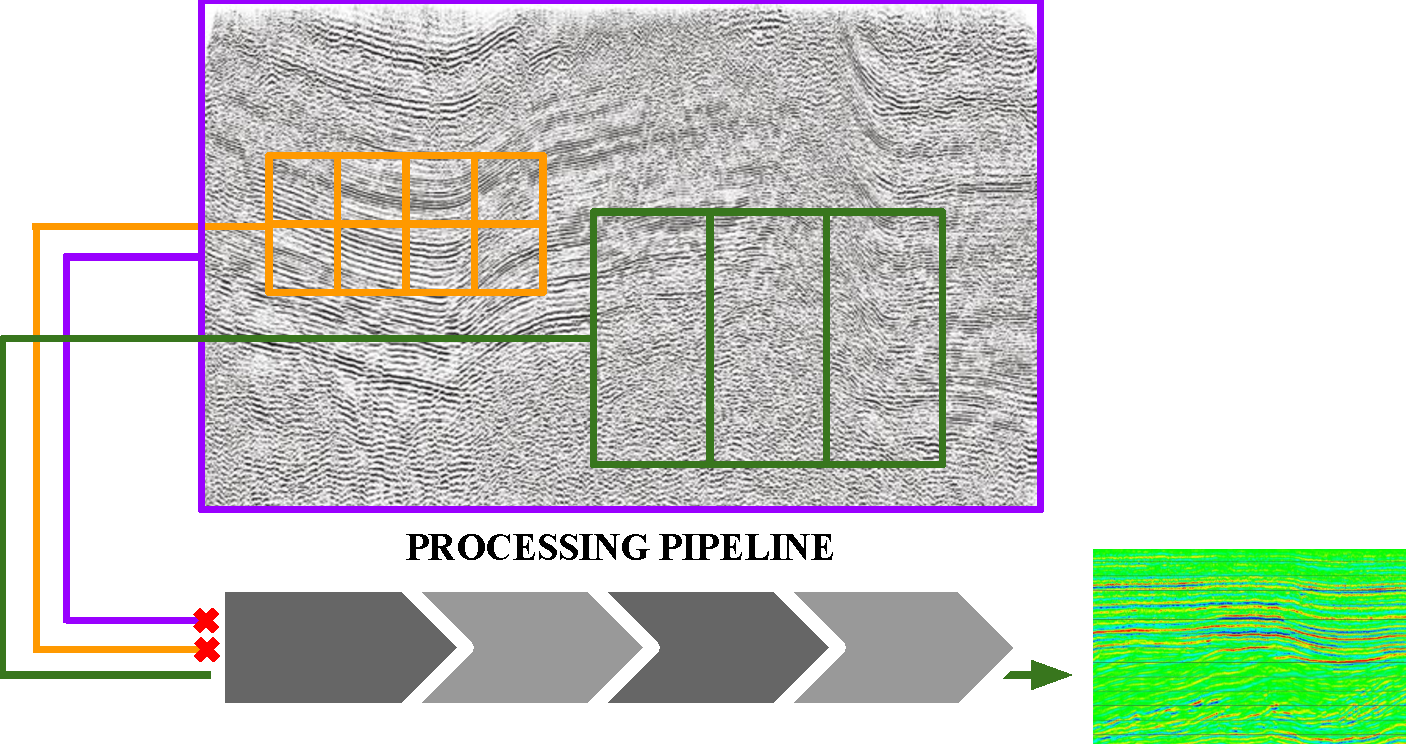
\includegraphics[width=0.95\textwidth]{assets/images/01/chunking-example}
    \caption{Example of seismic data chunking. Each colored rectangle indicates a potential chunk configuration, illustrating how different sizes and shapes can influence memory usage in the processing pipeline.}
    \label{fig:chunking-example}
\end{figure}

These challenges motivate the development of more reliable strategies for anticipating memory usage.
When the computation is memory-intensive, knowledge of memory requirements is critical, because one miscalculation can crash a job or underutilize the system.
In seismic processing, for instance, convolution-based algorithms or \ac{3D} filtering often exhibit unpredictable memory spikes due to short-lived but large intermediate arrays.
Therefore, a robust memory-aware method to define chunk dimensions is essential for \ac{HPC} and distributed systems, eliminating tedious attempts to guess resource allocations.


\section{Objectives}
\label{sec:intro-objectives}

The overarching objective of this thesis is to create a systematic and efficient method for estimating memory consumption in large-scale, Python-based data processing tasks, using a minimal number of experimental runs.
Specifically, the work seeks to integrate such predictive insights into Dask's chunking logic, making it memory-aware rather than relying on naive file-size or user-defined heuristics.

More concretely, this thesis pursues the following:
\begin{itemize}
    \item \textbf{Modeling Memory Usage.}
    Develop a procedure to profile Python's memory consumption in a controlled manner and derive a predictive model that correlates high-level input characteristics (\eg, volume or dimensional parameters) with peak memory usage.
    \item \textbf{Minimizing Trial Executions.}
    Ensure that profiling a small selection of data shapes or input sizes yields sufficient information to generalize memory demands across a broader range of workloads.
    \item \textbf{Enhancing Auto-Chunking.}
    Extend Dask's existing auto-chunking mechanism to account for memory requirements based on the model, reducing the risk of under-allocation or excessive overhead.
\end{itemize}


\section{Contributions}
\label{sec:intro-contributions}

The contributions of this thesis can be summarized as follows:
\begin{itemize}
    \item \textbf{Predictive Memory Model.}
    This thesis introduces a lightweight predictive model that estimates peak memory usage from a small set of profiler runs.
    The model exploits measurable input characteristics such as array dimensions and uses these as features in an empirically validated regression or \ac{ML} pipeline.

    \item \textbf{Practical Method for Minimal Profiling.}
    This thesis presents a method to reduce the profiling effort required, eliminating the need for multiple full-scale executions.
    The strategy isolates key data points or shapes to accurately capture operator memory behavior with minimal overhead, enabling more straightforward integration with real-world \ac{HPC} pipelines.

    \item \textbf{\traceq: A Memory Profiling Tool.}
    This thesis introduces \traceq, a lightweight library designed to collect memory usage traces with minimal overhead.
    It provides low-level logs and high-level visualizations of peak and intermediate memory consumption, assisting developers and researchers in identifying bottlenecks.
    In conjunction with the predictive model, \traceq simplifies and accelerates the creation of operator-specific memory profiles.

    \item \textbf{Memory-Aware Auto-Chunking.}
    The thesis proposes a memory-aware chunking algorithm that automatically sets chunk sizes in Dask using estimates from the predictive model.
    This approach reduces guesswork when partitioning data, mitigates \ac{OOM} failures, and avoids conservative over-allocation.

    \item \textbf{Real Seismic Data Case Study.}
    This thesis applies the proposed strategies to a large-scale seismic dataset, mirroring real-world industry requirements, in addition to theoretical and controlled evaluations.
    The experiments showcase the feasibility of the memory modeling approach and the advantages of memory-aware auto-chunking in a genuinely resource-intensive environment.
    Performance measurements and system logs confirm that the predictive model closely approximates actual memory consumption, substantially reducing the likelihood of \ac{OOM} incidents.
    Moreover, the results highlight how intelligently chosen chunk sizes improve throughput and overall utilization, ultimately validating the practical utility of this work in realistic seismic processing pipelines.
\end{itemize}

These developments address the critical need for robust memory management in high-volume seismic data processing and other demanding \ac{HPC} applications.
The solutions outlined here streamline distributed computing workflows that rely on Python and Dask for large-scale scientific or industrial tasks by combining measurement, modeling, and automated chunk resizing.


\section{Thesis Organization}
\label{sec:thesis-organization}

The remainder of this document consists of six chapters (Chapters~\ref{ch:fundamental-concepts}–\ref{ch:conclusion}) plus one appendix, each detailing a different aspect of this work.

Chapter~\ref{ch:fundamental-concepts} presents foundational material that clarifies how high-performance computing environments manage resources and concurrency.
It examines the principles behind data-intensive tasks and discusses seismic data characteristics, often creating heavy computational and memory demands.
It also describes Python's memory model, emphasizing the intricacies of garbage collection, fragmentation, and the differences between \ac{RSS} and \ac{VMS}.
Containerization practices like Docker and Singularity~\cite{singularity} appear next, explaining how \ac{cgroup} enforces memory limits and how nested containers affect measurement strategies.
This chapter closes by exploring data-parallel frameworks like Dask, where chunking decisions influence performance and reliability.

Chapter~\ref{ch:related-work} surveys the research on predictive memory management in high-performance and large-scale data-processing contexts.
It compares studies that help users specify job memory requirements more accurately and overviews algorithms for optimizing memory usage in frameworks like Apache Spark~\cite{zaharia2010spark}.
It then highlights gaps in the literature concerning robust and minimally invasive measurement strategies, providing a rationale for the approach pursued in subsequent chapters.

Chapter~\ref{ch:measuring-memory-consumption} focuses on accurately gauging Python's memory consumption.
It discusses pitfalls arising from dynamic allocation, container-level caching, and the overhead introduced by different profiling tools.
It demonstrates a recommended measurement strategy that ensures consistent and reliable peak-memory metrics.
This chapter also introduces the \traceq library, which automates and simplifies memory profile data collection.

Chapter~\ref{ch:predicting-memory-consumption-from-input-shapes} proposes a shape-based model that estimates peak memory usage from several carefully chosen profiler runs.
It explains the choice of input features, the process of collecting ground-truth data, and the empirical evaluation of multiple regression and machine learning methods.
The results reveal that a relatively small training dataset can produce an accurate model generalizing to broader workloads.
This chapter includes validation using both synthetic arrays and real seismic data.

Chapter~\ref{ch:improving-data-parallelism-using-memory-aware-chunking} builds on the predictive model by incorporating memory-aware chunking into Dask's existing auto-chunking mechanism.
It shows how chunk sizes adjust dynamically in response to anticipated memory demands.
It then compares this approach to default heuristics in a realistic seismic-processing scenario, demonstrating a reduction in \ac{OOM} incidents and improvements in the overall development process.

Chapter~\ref{ch:conclusion} summarizes key findings and discusses the primary contributions that emerge from measuring memory usage in Python, predicting peak consumption from input shapes, and integrating these insights into an automated chunking algorithm.
This closing chapter reiterates the significance of such techniques for large-scale seismic processing and similarly demanding applications.
It concludes by noting a few limitations of the current approach and suggesting extensions, such as expanded feature sets or integration with cluster-level schedulers.

Appendix~\ref{ch:appendix-challenges-pitfalls} contains more detailed discussions of the many practical challenges that complicate memory measurement in Python.
It examines additional experimental notebooks illustrating container-level effects, delayed garbage collection, and potential ways to mitigate measurement overhead.
This appendix offers deeper insights for practitioners who seek a more exhaustive analysis of memory profiling techniques.

These chapters progress from foundational concepts and a literature review through developing a predictive memory model to a practical demonstration of memory-aware chunking in a real-world seismic data scenario.
The thesis offers a cohesive approach to managing large-scale memory usage in Python-based \ac{HPC} applications by combining measurement techniques, modeling insights, and integration into a widely-used distributed framework.